\section{Auswertung}

\subsection{Fehlerrechnung}
Für die Auswertung müssen jeweils der Mittelwert einzelner Größen und seine Unsicherheit berechnet werden.
Die Formeln dazu sind im Folgenden angeben, wobei die individuellen Fehlerformeln für zusammengesetzte Größen im späteren Verlauf gesondert angegeben werden. 
Der Mittelwert $\bar{x}$ und seine Unsicherheit $\Del{\bar{x}}$ ergeben sich aus $N$ mal ermittelten Werten $x_i$, $i \in \mathbb{N}^{\leq N}$ durch
\begin{equation}
  \label{eq:mean}
  \bar{x} = \frac{1}{N} \sum_{i=1}^{N} x_i \qquad \text{und} \qquad \Del{\bar{x}} = \sqrt{ \frac{\sum_{i=1}^{N} \left( x_i - \bar{x} \right)^2}{N\,(N-1)}} \: .
\end{equation}

Setzt sich eine Größe $F$ aus $n$ fehlerbehafteten Größen $x_j$ zusammen, so berechnet sich der absolute Gauß-Fehler dieser Größe durch
\begin{equation}
  \label{eq:Gauss}
  \Del{F} = \sqrt{\sum_{j=1}^{n} \left( \frac{\partial F}{\partial x_j} \right)^2 (\Del{x_j})^2} \: .
\end{equation}

\subsection{Mittlere Weglängen}
Die mittleren Weglängen $\overline{w}$ lässt sich nach Gleichung (7) und (8) bestimmen.
Wichtig für die Messung ist das Verhältnis von dem Abstand zwischen Beschleunigungs- und Auffängerelektrode $a$ und der mittleren Weglänge $\overline{w}$.
Die berechneten Werte sind in Tabelle 1 aufgelistet, wobei $a = \SI{1 e-2}{\metre}$ beträgt.
\begin{table}[H]
    \begin{center}
      \begin{tabular}{c|c|c}
        \textbf{Temperatur T $[K]$} & \textbf{mittlere Weglänge $\overline{w}$ $[m]$} & \textbf{Verhältnis $\frac{a}{\overline{w}}$}\\
        \hline
        295.95 & 6.941 $\cdot$ $10^{-3}$ & 1.541 \\
        417.35 & 7.537 $\cdot$ $10^{-6}$ & 1.327 $\cdot$ $10^{3}$ \\
        433.15 & 4.132 $\cdot$ $10^{-6}$ & 2.420 $\cdot$ $10^{3}$ \\
        443.15 & 2.889 $\cdot$ $10^{-6}$ & 3.462 $\cdot$ $10^{3}$ \\
        456.25 & 1.850 $\cdot$ $10^{-6}$ & 5.406 $\cdot$ $10^{3}$ 
      \end{tabular}
      \caption{Die mittleren Weglängen für die verschiedenen Temperaturen und deren Verhältnis zu $a$.}
       \label{tab:mitt}
    \end{center}
\end{table}

  
Es wird deutlich dass das Verhältnis von $a$ und $\overline{w}$ mit steigender Temperatur deutlich größer wird.
Daraus kann eine höhere Sto\ss{}wahrscheinlichkeit gefolgert werden, da sich die Geschwindigkeit der Moleküle mit steigender Temperatur erhöht.

\subsection{Die Skala}
In diesem Abschnitt wird die Skala $S$ der Spannungs- bzw x-Achse bestimmt.
Ein Skalenanteil wird dabei als ein Centimeterkästchen definiert und die Spannung wird außerdem auf ein solches normiert.
\begin{table}[H]
  \begin{center}
    \label{tab:skala}
    \begin{tabular}{c|c|c}
       & \textbf{Spannungsbereich $[V]$} & \textbf{Skalenanteile $[Skt_x]$}\\
      \hline
                                  & (0-2) & 4.6 \\
                                  & (2-4) & 4.5 \\
      \textbf{Energieverteilung}  & (4-6) & 4.6 \\
                                  & (6-8) & 4.5 \\
                                  & (8-10) & 4.6\\
      \hline
                                    & (0-10) & 4.1 \\
                                    & (10-20) & 4.3 \\
      \textbf{Franck-Hertz-Kurven}  & (20-30) & 4.2 \\
                                    & (30-40) & 4.1 \\
                                    & (40-50) & 4.1 \\
                                    & (50-56) & 2.3 \\
      \hline
                                  & (0-5) & 3.8 \\
                                  & (5-10) & 3.9 \\
      \textbf{Ionisationsenergie} & (10-15) & 3.7 \\
                                  & (15-20) & 3.7 \\
                                  & (20-25) & 3.9 \\
                                  & (25-30) & 3.8
    \end{tabular}
    \caption{Die Skalen der Messreihen.}
  \end{center}
\end{table}

Nach Gleichung \ref{eq:mean} werden die Mittelwerte der Skalenanteile mit den abgelesenen Werten aus Tabelle 2 bestimmt.
Es ergeben für die verschiedenen Messungen folgende Skalenanteile.
\begin{equation}
  S_\text{x,E} = \SI{0.439 \pm 0.002}{\frac{V}{Skt_x}} \notag
\end{equation}
\begin{equation}
  S_\text{x,F} = \SI{2.429 \pm 0.032}{\frac{V}{Skt_x}} \notag
\end{equation}
\begin{equation}
  S_\text{x,I} = \SI{1.316 \pm 0.013}{\frac{V}{Skt_x}} \notag
\end{equation}
Dabei wurden die selben Skalierungen für jeweilige Messungen innerhalb eines Messbereichs verwendet.

\subsection{Energieverteilung}
In diesem Versuchsteil wird die integrale Energieverteilung bei einer konstanten Beschleunigungsspannung von $U_B = \SI{11}{V}$ und einer Temperatur von $T = \SI{295.95}{K}$ mittels eines x-y-Schreibers aufgezeichnet.
Durch Differenzierung dieser Funktion wird die differentielle Energieverteilung bestimmt.
Dazu werden Steigungsdreicke in das Diagramm eingezeichnet und die berechnete Steigung für verschiedene Spannungen in Tabelle 3 aufgelistet.

\begin{table}
  \label{tab:ener}
\begin{minipage}{0.5\textwidth}
  \begin{tabular}{c|c}
    \textbf{Spannung U $[V]$} & \textbf{Steigung $m$ $[\frac{A}{V}]$}\\
    \hline
    0.439 & 1.50 \\
    0.878 & 1.30 \\
    1.317 & 1.20 \\
    1.756 & 1.10 \\
    2.195 & 1.00 \\
    2.634 & 0.90 \\
    3.073 & 0.85 \\
    3.512 & 0.80 \\
    3.951 & 0.80 \\
    4.390 & 0.60 \\
    4.829 & 0.55 \\
    5.268 & 0.50 \\
    5.707 & 0.50 
  \end{tabular}
\end{minipage}
  \hfill
\begin{minipage}{0.75\textwidth} 
  \begin{tabular}{c|c}
    \textbf{Spannung U $[V]$} & \textbf{Steigung $m$ $[\frac{A}{V}]$}\\
    \hline
    6.146 & 0.45 \\
    6.585 & 0.40 \\
    7.024 & 0.35 \\
    7.463 & 0.35 \\
    7.902 & 0.30 \\
    8.078 & 0.25 \\
    8.341 & 0.34 \\
    8.561 & 0.4 \\
    8.780 & 0.5 \\
    8.868 & 1.0 \\
    8.912 & 1.5 \\
    9.000 & 0.5 \\
    9.131 & 0.34
  \end{tabular}
\end{minipage}
  \caption{Messwerte zur Steigung der eingezeichneten Steigungsdreiecke bei $T = \SI{295.95}{K}$.}
\end{table}

Nach der Normierung der maximalen Steigung ergibt sich die differentielle Energieverteilung, die in Abbildung \ref{fig:energ} aufgetragen ist.

\begin{figure}[h!]
  \centering
  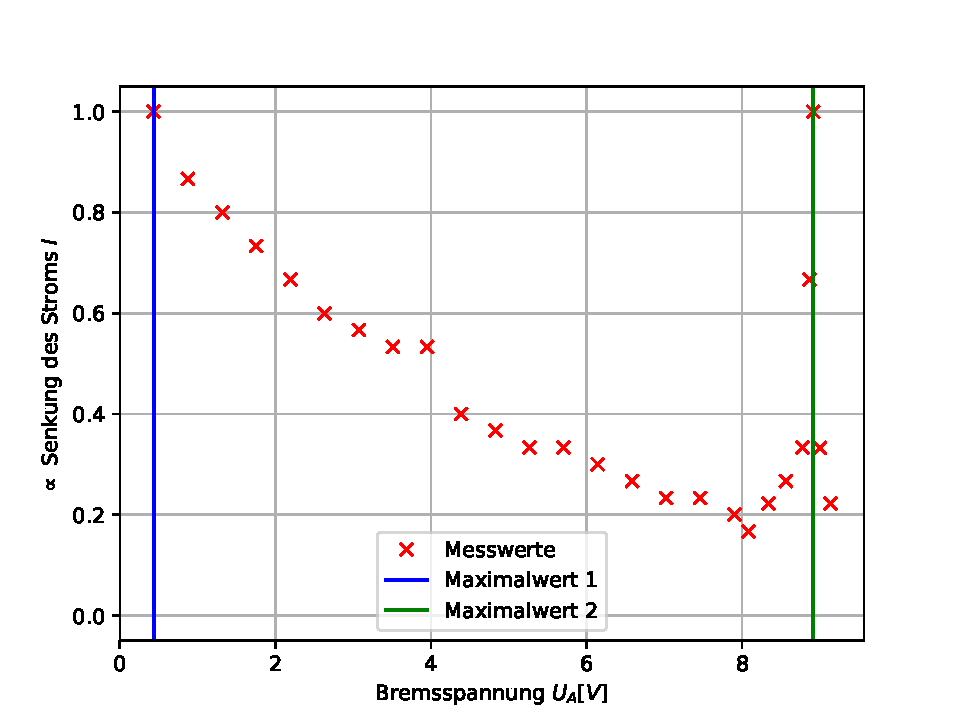
\includegraphics[height=8cm]{Auswertung/Steigung.pdf}
  \caption{Differentielle Energieverteilung bei $T = \SI{295.95}{K}$.}
  \label{fig:energ}
\end{figure}

Es werden Maxima bei $U_\text{max,1} = \SI{0.439}{V}$ und $U_\text{max,2} = \SI{8.912}{V}$ festgestellt.
Mittels Gleichung (9) lässt sich das Kontaktpotential $K$ nach
\begin{equation}
  K = U_B - U_\text{max}
\end{equation}
bestimmen.
Für die Kontaktpotentiale ergeben sich mit den abgelesenen Werten
\begin{equation}
  K_1 = \SI{10.561}{V} \qquad \text{und} \qquad K_2 = \SI{3.088}{V}.  \notag
\end{equation}
Physikalisch sinnvoll erscheint allerdings nur $K_2$, da $K_1$ praktisch im Verhältnis zur angelegenten Beschleunigungsspannung zu groß ist.

Die zweite Messung wurde bei einer Temperatur von $T = \SI{417.35}{K}$ und gleicher Beschleunigungsspannung aufgezeichnet.
Die dabei gemessenen Werte sind in Tabelle 4 aufgetragen.
\begin{table}
\label{tab:neu}
\centering
  \begin{tabular}{c|c}
    \textbf{Spannung U $[V]$} & \textbf{Steigung $m$ $[\frac{A}{V}]$}\\
    \hline
    0.351 & 1.00 \\
    0.790 & 1.00 \\
    1.229 & 0.94 \\
    1.668 & 0.88 \\
    2.107 & 0.83 \\
    2.546 & 0.78 \\
    2.985 & 0.72 \\
    3.424 & 0.61 \\
    3.863 & 0.44 \\
    4.302 & 0.37 \\
    4.565 & 0.09 \\
    (5-10) & 0.00  
  \end{tabular}
  \caption{Messwerte zur Steigung der eingezeichneten Steigungsdreiecke bei $T = \SI{417.35}{K}$}
\end{table}

\begin{figure}[h!]
  \centering
  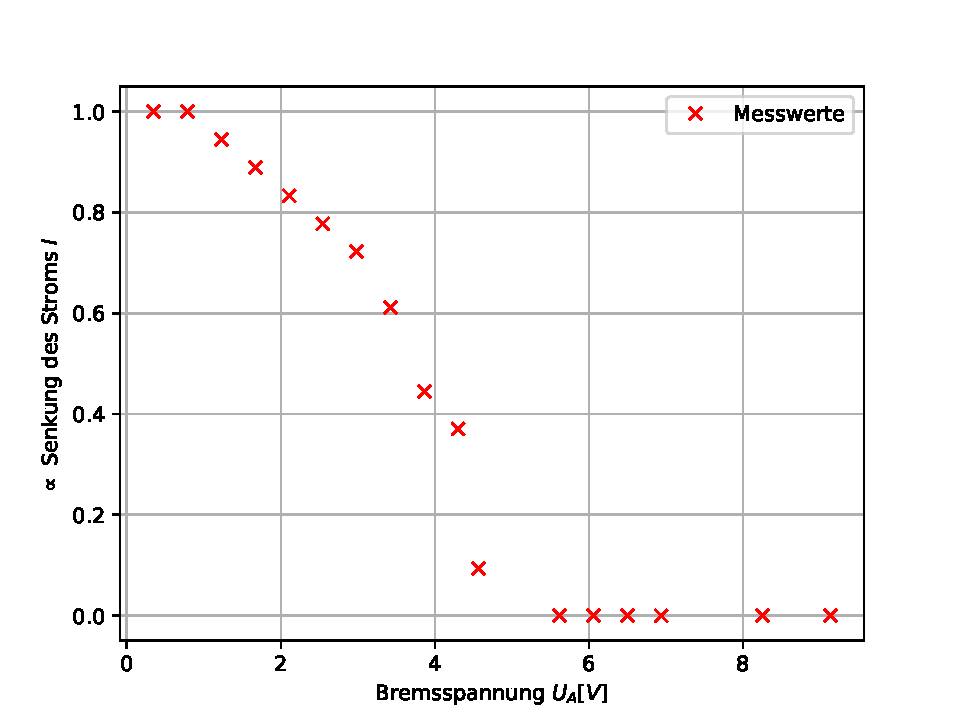
\includegraphics[height=8cm]{Auswertung/Steigung2.pdf}
  \caption{Differentielle Energieverteilung bei $T = \SI{417.35}{K}$.}
  \label{fig:energy}
\end{figure}
Die Abbildung \ref{fig:energy} zeigt die differentielle Energieverteilung für $T = \SI{417.35}{K}$.
Es wird deutlich, dass die integrale Energieverteilung schon bei kleineren Bremsspannungen ihr Minimum erreicht.
Die Elektronen verlieren also bei höheren Temperaturen bei Steigerung der Bremsspannung schneller ihre Energie.
Daraus lässt sich schließen, dass mehr Sto\ss{}prozesse stattfinden.

\subsection{Franck-Hertz Kurven}
Die Franck-Hertz Kurven weisen ein periodisch wiederkehrendes System auf.
Dabei werden die gemessenen Abstände zwischen den Maxima $U_1$ wie in Abbildung \ref{fig:Verlauf} abgelesen und in Tabelle 5 aufgelistet.

\begin{table}[H]
  \begin{center}
    \label{tab:franck}
    \begin{tabular}{c|c|c}
       & \textbf{Abstand der Maxima $[Skt_x]$} & \textbf{Abstand der Maxima $[V]$}\\
      \hline
                                    & 2.1 & 5.101 $\pm$ 0.067 \\
      \textbf{$T = \SI{433.15}{K}$} & 2.2 & 5.343 $\pm$ 0.070 \\
                                    & 2.2 & 5.344 $\pm$ 0.070 \\
      \hline
                                    & 2.0 & 4.858 $\pm$ 0.064 \\
                                    & 2.1 & 5.101 $\pm$ 0.067 \\
      \textbf{$T = \SI{443.15}{K}$} & 2.1 & 5.101 $\pm$ 0.067 \\
                                    & 2.2 & 5.344 $\pm$ 0.070 \\
                                    & 2.4 & 5.830 $\pm$ 0.077 \\
      \hline
                                    & 2.0 & 4.858 $\pm$ 0.064 \\
                                    & 2.1 & 5.101 $\pm$ 0.067 \\
      \textbf{$T = \SI{456.25}{K}$} & 2.1 & 5.101 $\pm$ 0.067 \\
                                    & 2.2 & 5.344 $\pm$ 0.070 \\
                                    & 2.3 & 5.587 $\pm$ 0.074
    \end{tabular}
    \caption{Abstand der Maxima bei den Franck-Hertz Kurven für die verschiedenen Temperaturen.}
  \end{center}
\end{table}

Aus Gleichung \ref{eq:mean} wird dann der Mittelwert und der dazugehörige Fehler bestimmt und es ergibt sich
\begin{equation}
  \overline{U_1} = \SI{5.232 \pm 0.076}{V}. \notag
\end{equation}

Anschließend wird nach Gleichung (6) das Anregungspotential der Quecksilber-Atome auf
\begin{equation}
  E_1 - E_0 = e_0 U_1 = \SI{5.232 \pm 0.076}{eV} = \SI{8.371 \pm 0.122}{10^{-19} J} \notag
\end{equation}
berechnet.
Zusätzlich wird die Wellenlänge mittels Gleichung (5) und des Zusammenhangs $\lambda = \frac{c}{\nu}$ auf
\begin{equation}
  \lambda = \frac{h \; c}{E_1-E_0} = \SI{237.151 \pm 3.440}{nm} \notag
\end{equation}
bestimmt.
Das emittierte Licht liegt somit noch im Ultravioletten Bereich.
Beim zentral elastischen Sto\ss{} kann aufgrund der hohen Massendifferenz der beiden Stoßpartner davon ausgegangen werden, dass das Elektron nahezu keine Energie verliert und somit nur eine Richtungsänderung erfährt.
So kann das Elektron bei dem nächsten Sto\ss{} ein Hg-Atom anregen.
Somit muss bei der Auswertung der Energieverlust beim zentral elastischen Stoss{} nicht berücksichtigt werden.

\subsection{Ionisierungsenergie}
Zur Bestimmung der Ionisationsenergie wird die Nullstelle mittels einer linearen Regression der Form
\begin{equation}
  y = m \cdot x \notag
\end{equation}
berechnet.
Dazu wird die Messung mit einer negativen Bremsspannung von $U_A = \SI{-30}{V}$ verwendet und das nahezu lineare Ende der Messkurve genähert.
Die abgelesenen Werte sind in Tabelle 5 aufgelistet.

\begin{table}[H]
  \begin{center}
    \label{tab:ion}
    \begin{tabular}{c|c}
      \textbf{Spannung $U_B [V]$} & \textbf{Strom I (normiert)}\\
      \hline
      21.056 $\pm$ 0.208 & 0.219 \\
      21.714 $\pm$ 0.215 & 0.258 \\
      22.372 $\pm$ 0.221 & 0.290 \\
      23.030 $\pm$ 0.227 & 0.335 \\
      23.688 $\pm$ 0.234 & 0.380 \\
      23.346 $\pm$ 0.241 & 0.425 \\
      25.004 $\pm$ 0.247 & 0.471 \\
      25.662 $\pm$ 0.254 & 0.529 \\
      26.320 $\pm$ 0.260 & 0.587 \\
      26.978 $\pm$ 0.267 & 0.645 \\
      27.636 $\pm$ 0.273 & 0.716 \\
      28.294 $\pm$ 0.280 & 0.787 \\
      28.952 $\pm$ 0.286 & 0.865 \\
      29.610 $\pm$ 0.293 & 0.935 \\
      30.268 $\pm$ 0.299 & 1
    \end{tabular}
    \caption{Der normierte Strom in Abhängigkeit von der Beschleunigungsspannung für $T = \SI{417.35}{K}$.}
  \end{center}
\end{table}

Die lineare Regression aus Abbildung \ref{fig:ion} liefert mittels Bestimmung der Parameter die Nullstelle
\begin{equation}
  U_0 = U_\text{Ion} + K = \SI{19.099 \pm 0.1}{V}. \notag
\end{equation}

Mit dem Kontaktpotential aus dem Abschnitt Energieverteilung ergibt sich für die Ionisationsenergie
\begin{equation}
  E_\text{Ion} = e_0 \; (U_0 - K) = \SI{16.011 \pm 0.2}{eV}. \notag
\end{equation}

\begin{figure}[h]
  \centering
  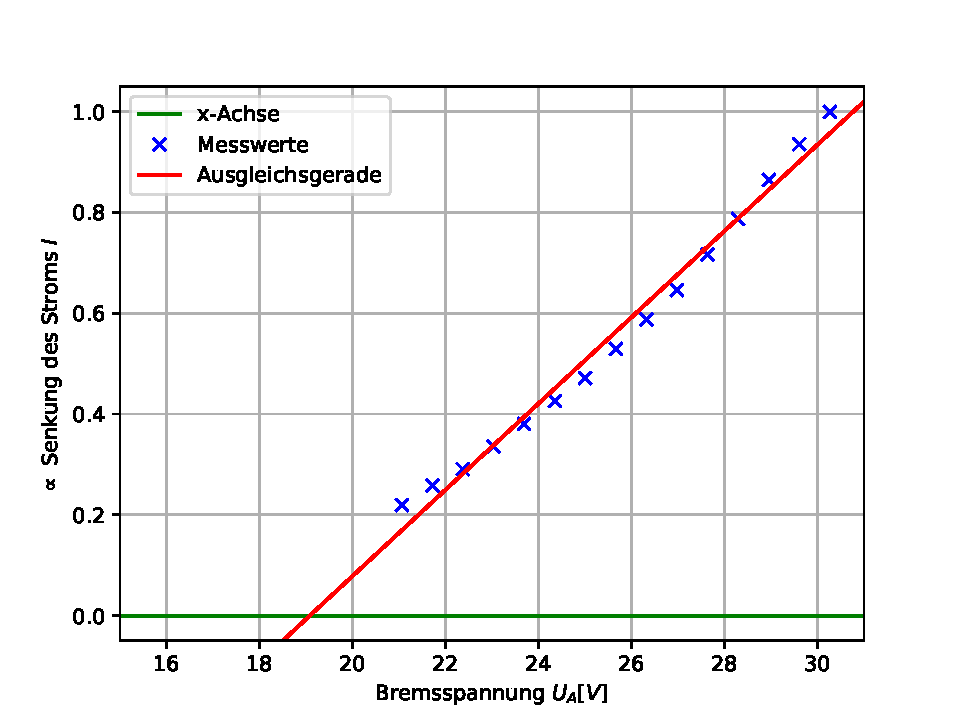
\includegraphics[height=8cm]{Auswertung/regression.pdf}
  \caption{Lineare Regression zur Bestimmung der Ionisationsenergie.}
  \label{fig:ion}
\end{figure}
